\documentclass[]{article}

%packages
\usepackage[utf8]{vietnam}
\usepackage{amsmath, amssymb, amsthm}
\usepackage{graphicx, caption}
\everymath{\displaystyle}
%opening
\title{}
\author{}

\begin{document}

%\maketitle

%\begin{abstract}
%
%\end{abstract}

\section{Supervised learning - classification}
\noindent \textbf{Ký hiệu:}
\begin{itemize}
	\item $m$ là số mẫu và $n$ là số thành phần dữ liệu.
	\item $x, x_{ij}\in \mathbb{R}$ là các số thực.
	\item $\textbf{x},\, \textbf{x}_i =\left(x_{i1}, x_{i2},\cdots, x_{im}\right)^T \in \mathbb{R}^{m\times 1}$ là các vector.
	\item $\textbf{X}=[\textbf{x}_1, \textbf{x}_2, \cdots, \textbf{x}_n]\in \mathbb{R}^{m\times n}$ là ma trận $m\times n$.
\end{itemize}
\subsection{Supervised learning}
\textbf{Supervised learning} (học có giám sát) là thuật toán dự đoán đầu ra của một dữ liệu mới dựa trên các dữ liệu và đầu ra tương ứng đã biết từ trước. Tức là khi chúng ra có một tập hợp biến đầu vào $\mathcal{X} = \{\mathbf{x}_1, \mathbf{x}_2, \dots, \mathbf{x}_n\}$ và một tập hợp đầu ra tương ứng $\mathcal{Y} = \{\mathbf{y}_1, \mathbf{y}_2, \dots, \mathbf{y}_n\}$, trong đó $\mathbf{x}_i, \mathbf{y}_i$ là các vector. Các cặp dữ liệu biết trước $(\mathbf{x}_i, \mathbf{y}_i) \in \mathcal{X} \times \mathcal{Y}$ được gọi là training data (tập dữ liệu huấn luyện). Từ tập dữ liệu huấn luyện này, chúng ta xác định một hàm $f:\mathcal{X}\to \mathcal{Y}$ sao cho
$$\hat{\mathbf{y}}_i = f(\mathbf{x}_i) \approx \textbf{y}_i, ~~ \forall i = 1, 2, \dots, n.$$
Mục đích là xấp xỉ hàm số $f$ thật tốt để khi có một dữ liệu 
$\mathbf{x}$ mới, chúng ta có thể tính đầu ra $\textbf{y}=f(\textbf{x})$ tương ứng của nó.

\subsection{Classification}
Một trong những bài toán thuộc supervised learning là \textbf{classification} (phân loại). Tức là đầu ra là các nhãn và $\mathcal{Y}$ là một tập hữu hạn các nhãn. Trong bài cáo này, em chỉ xét bài toán binary classification, tức là bài toán chỉ có hai nhãn, cụ thể $\mathcal{Y}=\{0,\,1\}$. Ví dụ của bài toán: Xác định xem một khối u có phải là ác tính hay lành tính; Gmail xác định xem một email có phải là spam hay không.

\subsection{Feature engineering}
Các thành phần dữ liệu đôi khi được đo đạc với những đơn vị khác nhau hoặc có giá trị chênh lệch nhau quá lớn sẽ ảnh hưởng đến thuật toán, ví dụ tốc độ hội tụ của Gradient Descent sẽ lâu hơn. Giả sử $\textbf{x}$ là vectơ giá trị ban đầu, $\textbf{x}'$ là vectơ giá trị sau khi chuẩn hóa, chúng ta có những phương pháp thông dụng sau đây:
\subsubsection{Rescaling}
Phương pháp đơn giản nhất là đưa tất cả các thành phần về cùng một khoảng $[0, 1]$
hoặc $[-1, 1]$ chẳng hạn, tùy thuộc vào bài toán. Nếu muốn chuẩn hóa dữ liệu về khoảng $[0, 1]$:
$$\textbf{x}' = \frac{\textbf{x} - \min(\textbf{x})}{\max(\textbf{x}) - \min(\textbf{x})}.$$
\subsubsection{Mean normalization}
Phương pháp này sẽ chuẩn hóa dữ liệu về dữ liệu có các thành phần với kỳ vọng $0$ và giá trị thuộc khoảng $[-0.5, 0.5]$:
$$\textbf{x}' = \frac{\textbf{x} - \text{mean}(\textbf{x})}{\max(\textbf{x}) - \min(\textbf{x})},$$
với $\text{mean}(\textbf{x})$ lần lượt là kỳ vọng thành phần dữ liệu đó.
\subsubsection{Standardization}
Một phương pháp nữa cũng hay được sử dụng, giả sử mỗi thành phần đều có phân phối chuẩn với kỳ vọng là $0$ và phương sai là $1$:
$$\textbf{x}' = \frac{\textbf{x} - \text{mean}(\textbf{x})}{\text{std}(\textbf{x})}$$
với $\text{mean}(\textbf{x}),\, \text{std}(\textbf{x})$ lần lượt là kỳ vọng và phương sai của thành phần dữ liệu đó.

\subsection{Overfitting}
Overfitting là hiện tượng mô hình tìm được quá khớp với dữ liệu training.  Việc quá khớp này có thể dẫn đến việc dự đoán nhầm nhiễu, và chất lượng mô hình không còn tốt trên dữ liệu test nữa.
\subsubsection{Phân loại dữ trên overfitting}
\textbf{Train error}: Thường là hàm mất mát áp dụng lên training data. Hàm mất mát này cần có một thừa số $\frac{1}{m_{\text{train}}}$ để tính giá trị trung bình, tức mất mát trung bình trên mỗi điểm dữ liệu:
$$\text{error}_{\text{train}}= \frac{1}{m_{\text{train}}} \sum_{\text{training set}} g(y-\hat{y}).$$
\textbf{Test error}: Tương tự như trên nhưng áp dụng mô hình tìm được vào test data. Chú ý rằng, khi xây dựng mô hình, ta không được sử dụng thông tin trong tập dữ liệu test. Dữ liệu test chỉ được dùng để đánh giá mô hình:
$$\text{error}_{\text{test}}= \frac{1}{m_{\text{test}}} \sum_{\text{test set}} g(y-\hat{y}).$$
Việc lấy trung bình là quan trọng vì lượng dữ liệu trong hai tập hợp training và test có thể chênh lệch rất nhiều.
\begin{center}
	\begin{tabular}{ |c|c|c|c| } 
		\hline
		$\text{error}_{\text{train}}$ & thấp & thấp & cao\\
		\hline 
		$\text{error}_{\text{test}}$ & thấp & cao&cao \\ 
		\hline
		Mô hình& fit (tốt) & overfitting &underfitting\\ 
		\hline
	\end{tabular}
\end{center}
%Một mô hình được coi là tốt nếu cả $\text{error}_{\text{train}}$ và $\text{error}_{\text{test}}$ đều thấp. Nếu $\text{error}_{\text{train}}$ thấp nhưng $\text{error}_{\text{test}}$ cao, ta nói mô hình bị overfitting. Nếu train error cao và $\text{error}_{\text{test}}$ cao, ta nói mô hình bị underfitting.
\subsubsection{Phương pháp tránh overfitting}
Chúng ta có phương pháp thông dụng sau đây:
\begin{itemize}
	\item \textbf{Reduce number of features}:
	\begin{itemize}
		\item Loại bỏ những thành phần không hoặc có ít ảnh hưởng đến kết quả.
		\item Chọn mô hình phù hợp với bài toán.
	\end{itemize}
	\item \textbf{Regularization}:
	\begin{itemize}
		\item Giữ lại tất cả các thành phần, nhưng thay đổi giá trị trọng số $\theta$.
		\item Phương pháp này vẫn tốt ngay cả khi có rất nhiều thành phần dữ liệu mà mỗi thành phần chỉ góp một ít vào kết quả dự đoán.
	\end{itemize}
\end{itemize}
Trong bài báo cáo này, em sẽ sử dụng phương pháp regularization.
\subsubsection{Regularization}
Regularization một cách cơ bản là thay đổi mô hình một chút để tránh overfitting trong khi vẫn giữ được tính tổng quát của nó (tính tổng quát là tính mô tả được nhiều dữ liệu, trong cả tập training và test). Một cách cụ thể hơn, ta sẽ tìm cách di chuyển nghiệm của bài toán tối ưu hàm mất mát tới một điểm gần nó. Hướng di chuyển sẽ là hướng làm cho mô hình ít phức tạp hơn mặc dù giá trị của hàm mất mát có tăng lên một chút.
\\
Kỹ thuật regularization phổ biến nhất là thêm vào loss function (hàm mất mát) một số hạng nữa. Số hạng này thường dùng để đánh giá độ phức tạp của mô hình. Số hạng này càng lớn, thì mô hình càng phức tạp. Hàm mất mát mới này thường được gọi là regularized loss function, thường được định nghĩa như sau:
$$J_{\lambda}(\theta) = J(\theta) + \lambda R(\theta)\to \min,$$
với $\theta\in \mathbb{R}^{n\times 1}$ là weight (trọng số) và $\lambda>0$ được gọi là tham số regularization. Trong bài báo cáo này, em chọn hàm thêm vào $R(\theta)$ có dạng
$$R(\theta)=\sum_{j=1}^{n}\theta_j^2.$$
Lưu ý, $\lambda$ thường được chọn là một số nhỏ để biểu thức regularization không làm giảm quá nhiều đến nghiệm thu được so với nghiệm gốc. Nhưng nếu $\lambda$ quá lớn thì dẫn đến mô hình thu được bị underfitting. Ví dụ $J_{\lambda}(\theta)=\theta_0+\theta_1\textbf{x}_1 +\theta_2\textbf{x}_2+\lambda (\theta_1^2+\theta_2^2)\to \min$, dẫn đến $(\theta_1, \theta_2)=(0, 0)$.

\subsection{Gradient Descent}
\subsubsection{Gradient Descent một biến}
Xét bài toán $$f(x)=\frac{1}{2}(x-2)^2-2\to \min.$$
\begin{figure}[h!]
	\centering
	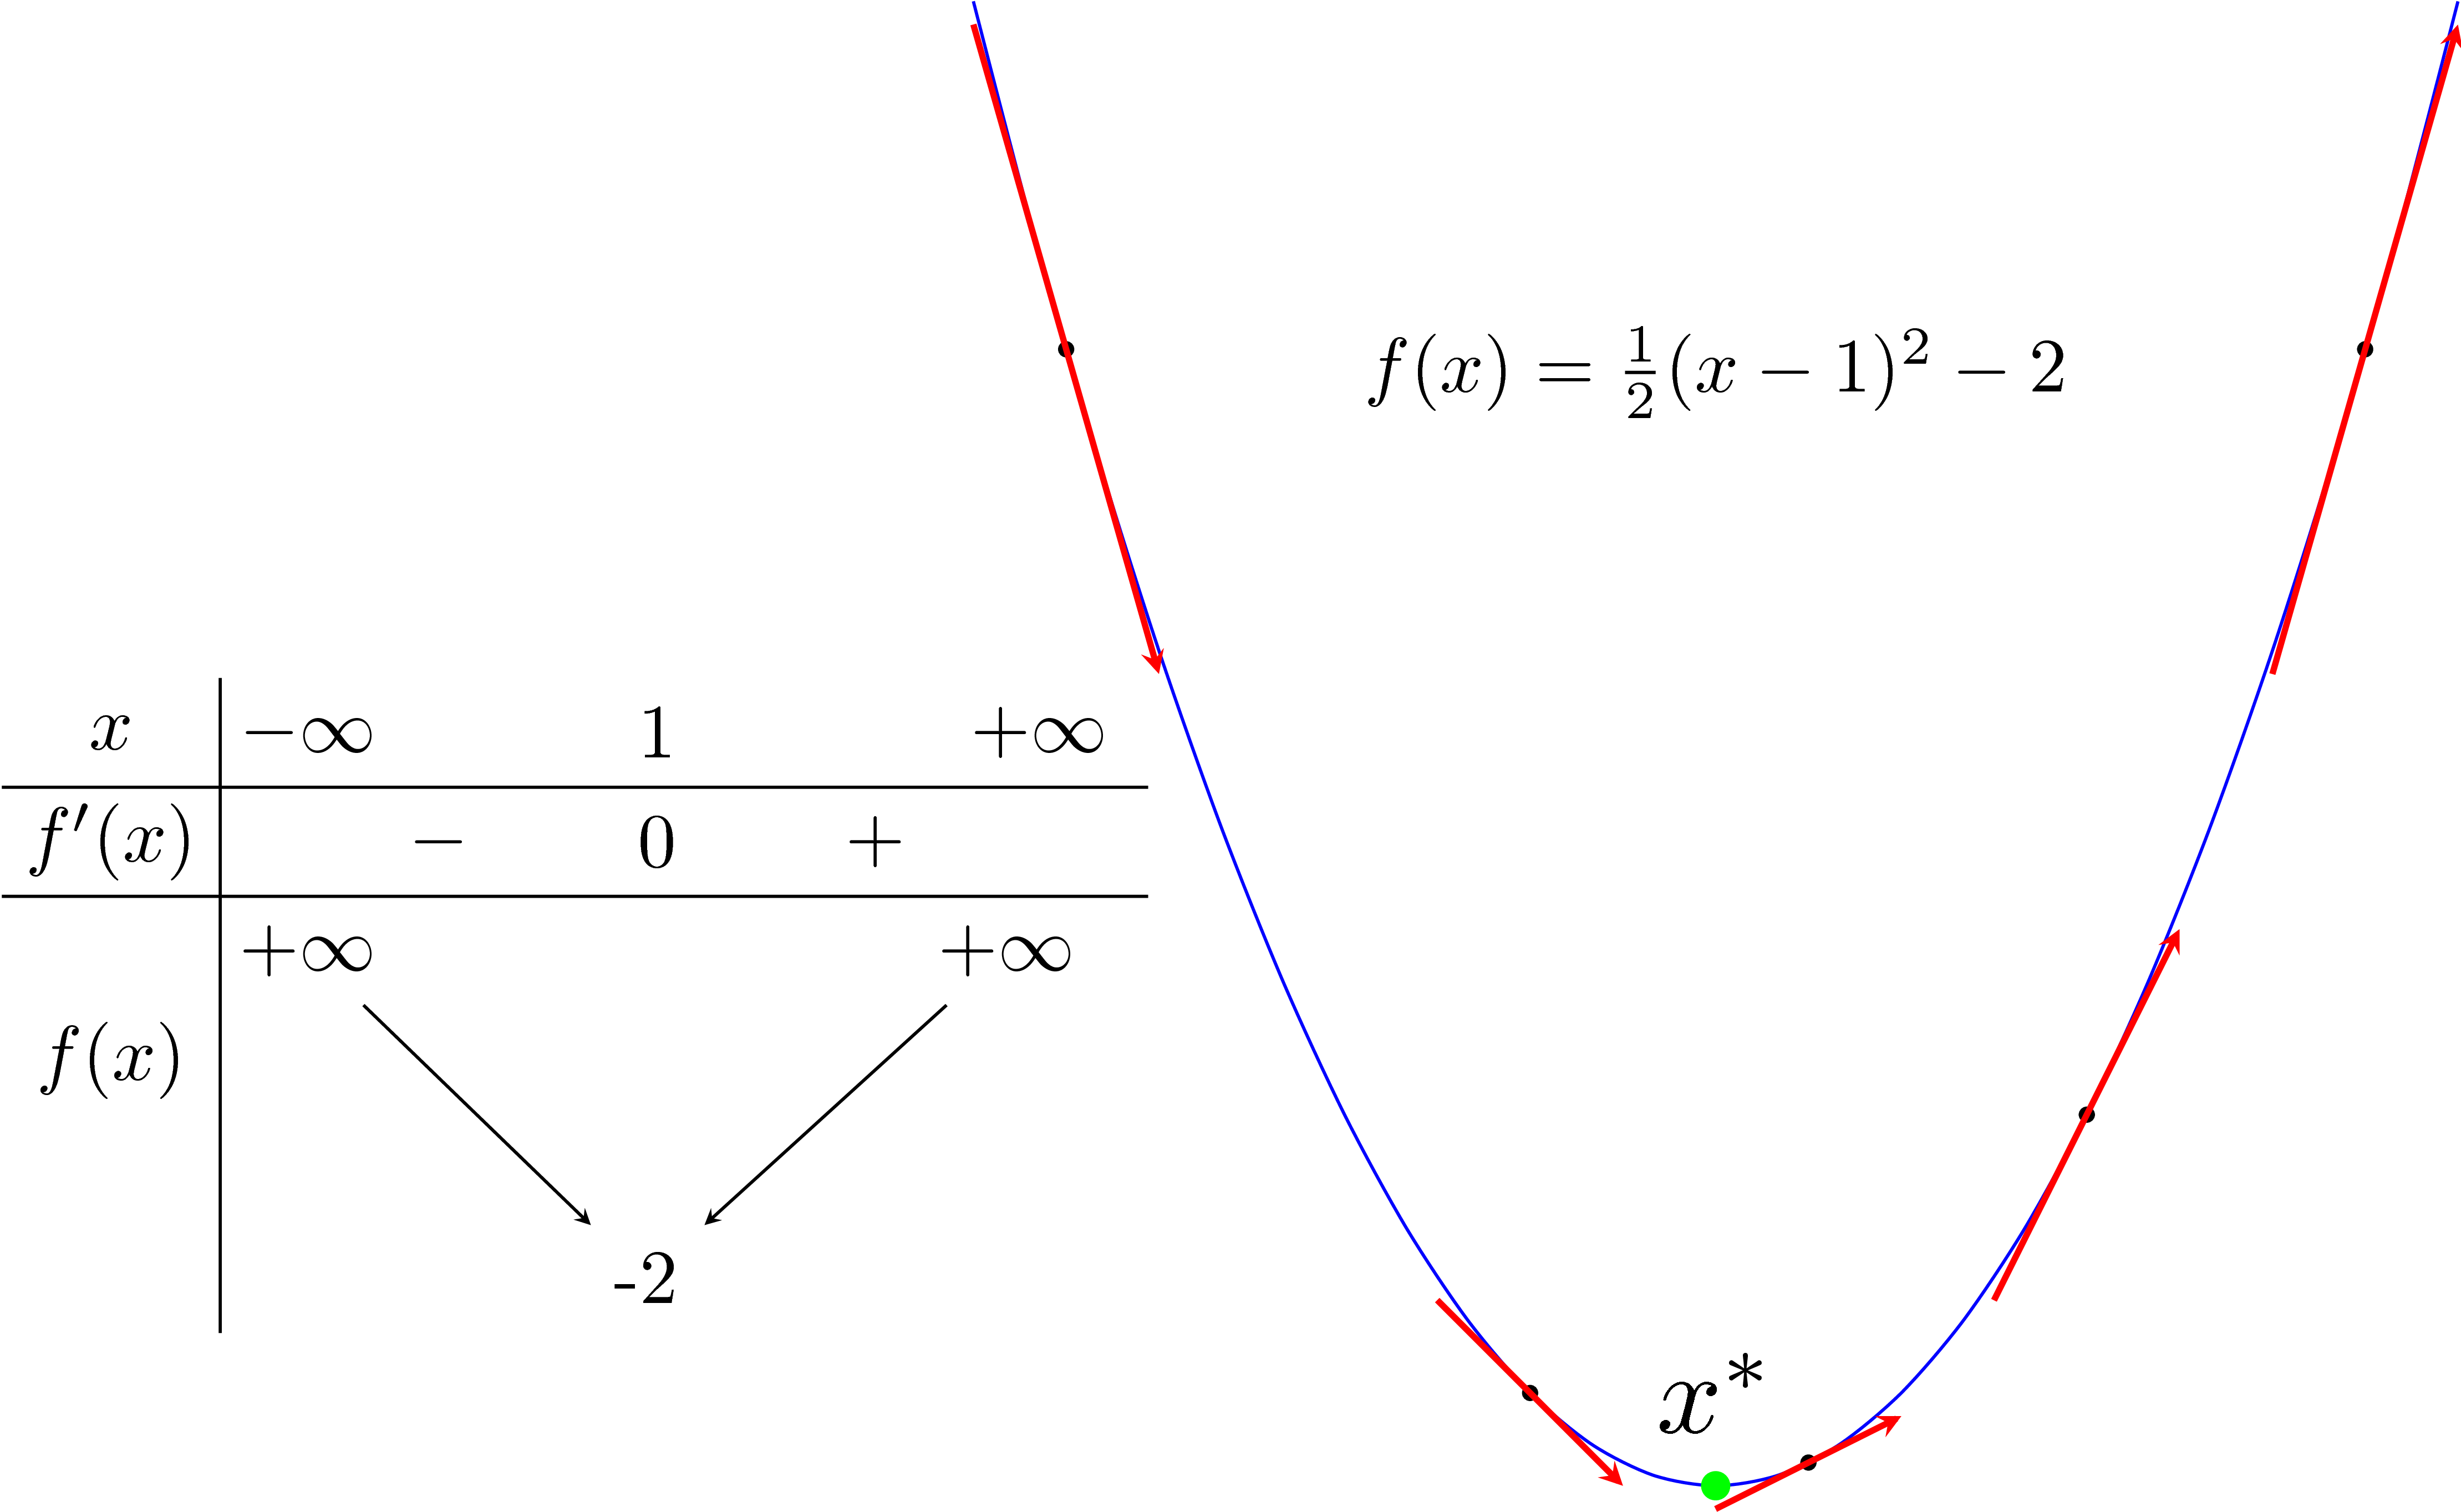
\includegraphics[width=0.8\linewidth]{gradient_descent}
	\caption{Bảng khảo sát hàm số và đồ thị hàm $f(x)$}
\end{figure}
\noindent Giả sử $x^*$ là nghiệm của bài toán trên và $x_t$ là điểm ta tìm được sau vòng lặp thứ $t$. Ta cần tìm một thuật toán để đưa $x_t$ về càng gần $x^*$ càng tốt.
\\
Trong hình đầu tiên, chúng ta lại có thêm hai quan sát nữa:
\begin{itemize}
	\item Nếu đạo hàm của hàm số tại $x_t:\, f'(x_t)>0$ thì $x_t$ 	nằm về bên phải so với $x^*$ (và ngược lại). Để điểm tiếp theo $x_{t+1}$ gần với $x^*$ hơn, chúng ta cần di chuyển $x_t$ về phía bên trái, tức về phía âm. Nói các khác, chúng ta cần di chuyển ngược dấu với đạo hàm:
	$$x_{t+1} = x_{t} + \Delta,$$
	trong đó $\Delta$ là một đại lượng ngược dấu với đạo hàm $f'(x_t)$.
	\item Nếu $x_t$ càng xa $x^*$ về phía bên phải thì $f'(x_t)$ càng lớn hơn 0 (và ngược lại). Vậy, lượng di chuyển $\Delta$ một cách trực quan nhất, là tỉ lệ thuận với $-f'(x_t)$.
\end{itemize}
Hai nhận xét phía trên cho chúng ta một cách cập nhật đơn giản là:
$$x_{t+1} = x_{t} - \eta f’(x_{t}).$$
Trong đó $\eta$ là một số dương được gọi là learning rate (tốc độ học). Dấu trừ thể hiện việc chúng ta phải đi ngược với đạo hàm.

\subsubsection{Gradient Descent nhiều biến}
Giả sử ta cần tìm $\theta^*=\arg\min_{\theta}f(\theta)$, trong đó $\theta$ là một vector, thường được dùng để ký hiệu tập hợp các tham số của một mô hình cần tối ưu. Đạo hàm của hàm số đó tại một điểm $\theta$ bất kỳ được ký hiệu là $\nabla_\theta J(\theta)$. Tương tự như hàm 1 biến, thuật toán GD cho hàm nhiều biến cũng bắt đầu bằng một điểm dự đoán $\theta_0$, sau đó, ở vòng lặp thứ $t$, quy tắc cập nhật là:
$$\theta_{t+1} = \theta_{t} - \eta \nabla_{\theta} f(\theta_{t}),$$
hay viết dưới dạng đơn giản
$$\theta = \theta - \eta \nabla_{\theta} f(\theta).$$
\subsubsection{Gradient Descent với momentum}
\textit{\textbf{Gradient dưới góc nhìn vật lý}}
\\
Thuật toán GD thường được ví với tác dụng của trọng lực lên một hòn bi đặt trên một mặt có dạng như hình một thung lũng giống như hình 1a) dưới đây. Bất kể ta đặt hòn bi ở A hay B thì cuối cùng hòn bi cũng sẽ lăn xuống và kết thúc ở vị trí C.
\begin{figure}[h!]
	\centering
	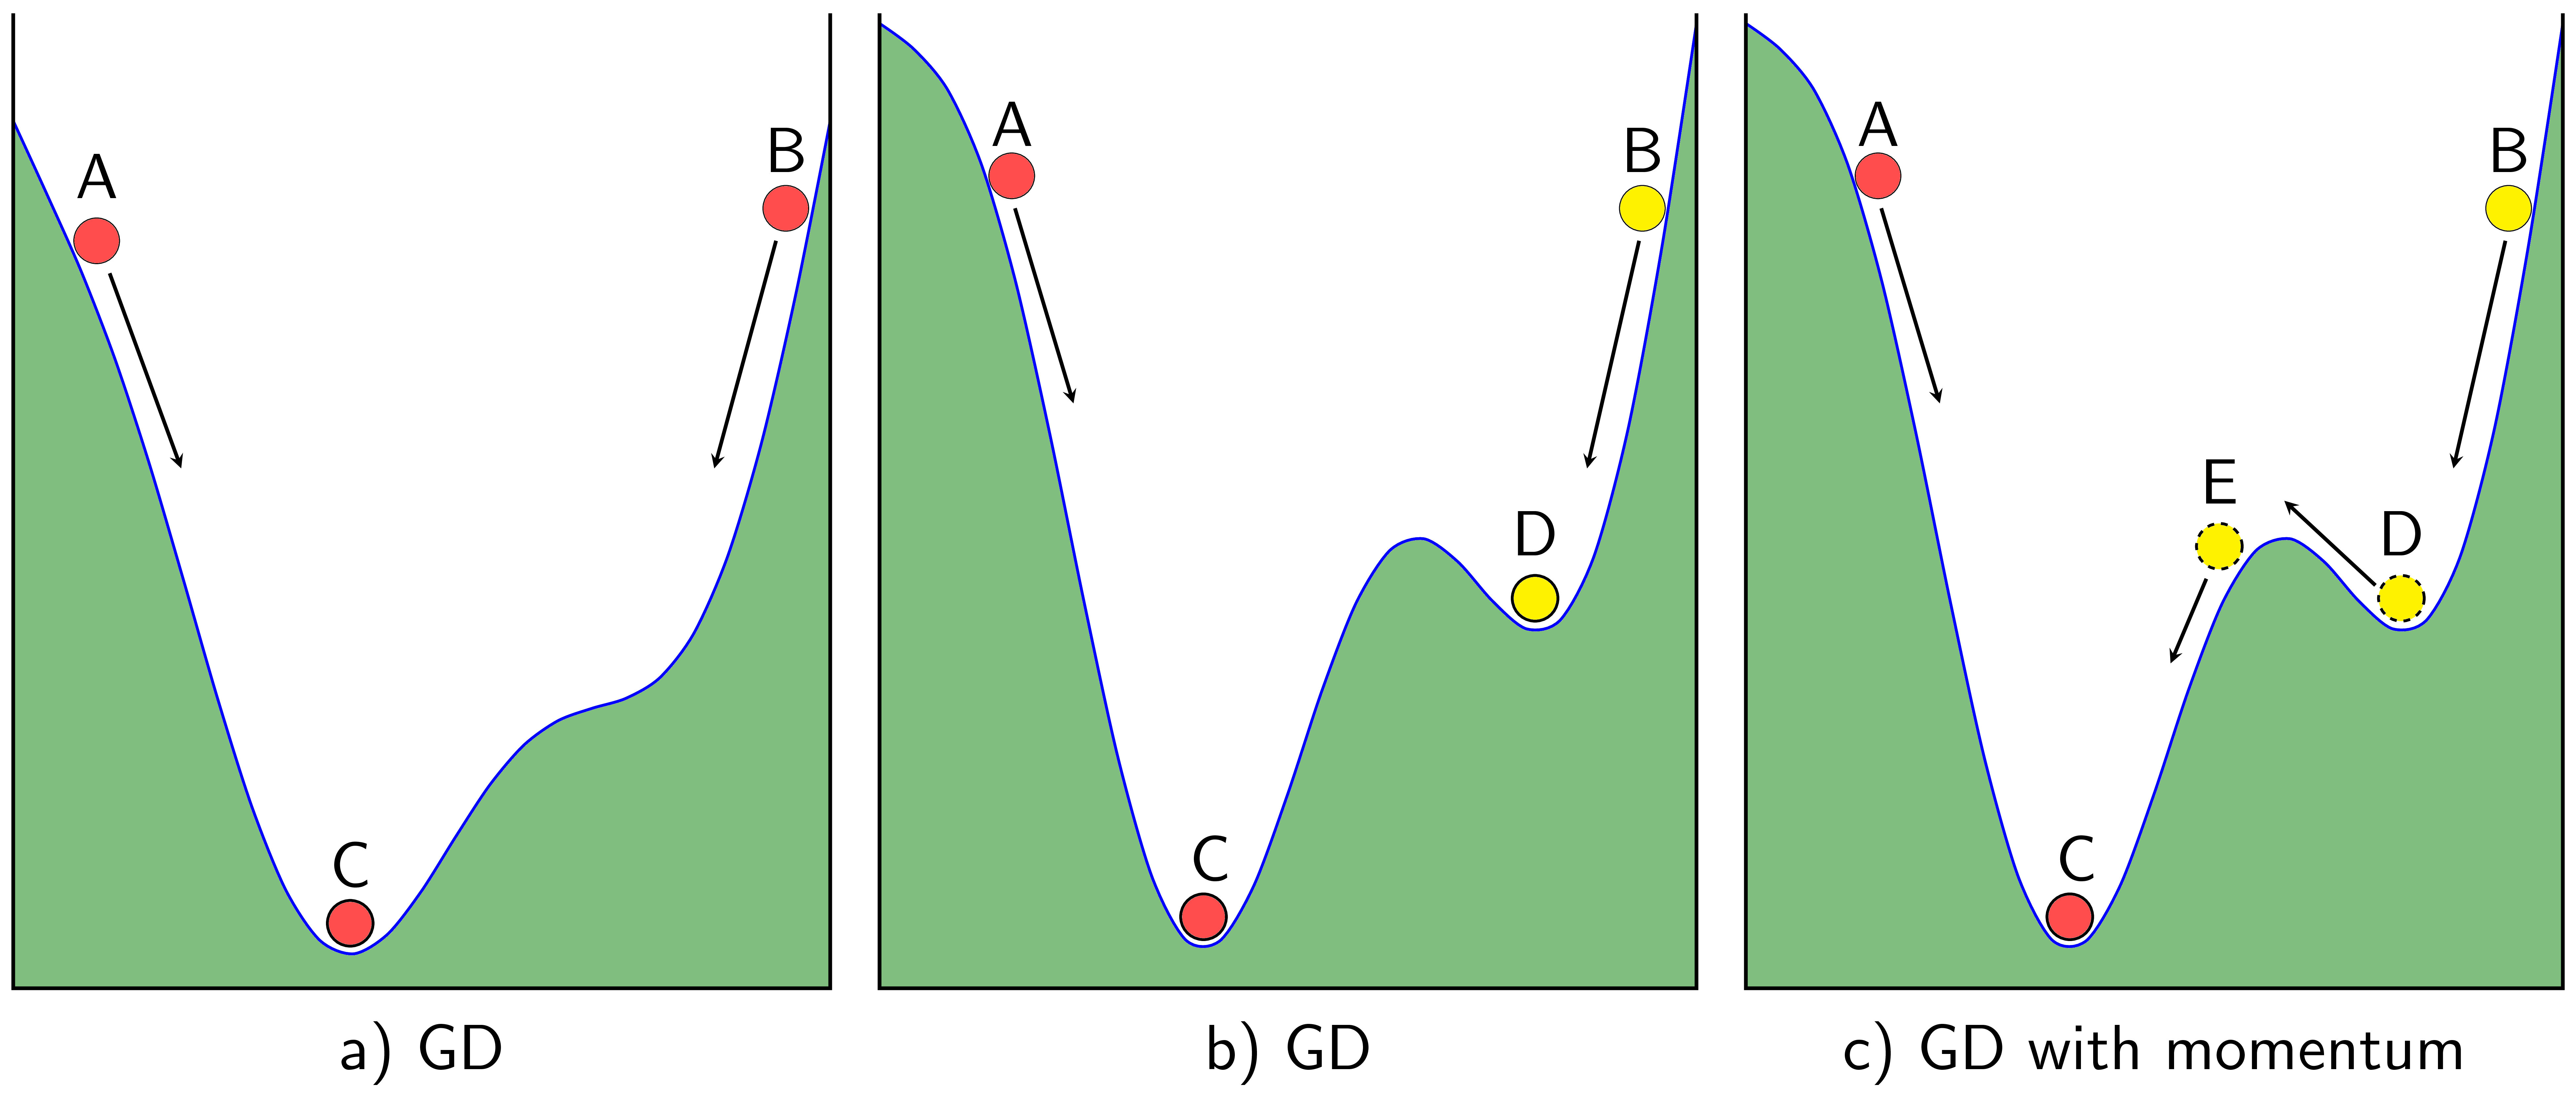
\includegraphics[width=0.9\linewidth]{momentum}
	\caption{So sánh Gradient Descent với các hiện tượng vật lý}
\end{figure}

\noindent Tuy nhiên, nếu như bề mặt có hai đáy thung lũng như Hình 1b) thì tùy vào việc đặt bi ở A hay B, vị trí cuối cùng của bi sẽ ở C hoặc D. Điểm D là một điểm local minimum chúng ta không mong muốn.
\\
Nếu suy nghĩ một cách vật lý hơn, vẫn trong Hình 1b), nếu vận tốc ban đầu của bi khi ở điểm B đủ lớn, khi bi lăn đến điểm D, theo đà, bi có thể tiếp tục di chuyển lên dốc phía bên trái của D. Và nếu giả sử vận tốc ban đầu lớn hơn nữa, bi có thể vượt dốc tới điểm E rồi lăn xuống C như trong Hình 1c). Đây chính là điều chúng ta mong muốn. 
\\
Dựa trên hiện tượng này, một thuật toán được ra đời nhằm khắc phục việc nghiệm của GD rơi vào một điểm local minimum không mong muốn. Thuật toán đó có tên là Momentum.
\\\\
\textit{\textbf{Gradient Descent với Momentum}}
\\
Trong GD, chúng ta cần tính lượng thay đổi ở thời điểm $t$ để cập nhật vị trí mới cho nghiệm (tức hòn bi). Nếu chúng ta coi đại lượng này như vận tốc $v_t$ trong vật lý, vị trí mới của hòn bi sẽ là $\theta_{t+1} = \theta_{t} - v_t$. Dấu trừ thể hiện việc phải di chuyển ngược với đạo hàm. Công việc của chúng ta bây giờ là tính đại lượng $v_t$ sao cho nó vừa mang thông tin của độ dốc (tức đạo hàm), vừa mang thông tin của đà, tức vận tốc trước đó $v_{t-1}$(chúng ta coi như vận tốc ban đầu $v_0=0$). Một cách đơn giản nhất, ta có thể cộng (có trọng số) hai đại lượng này lại:
$$v_{t}= \gamma v_{t-1} + \eta \nabla_{\theta}J(\theta),$$
trong đó $\gamma$ thường được chọn là một giá trị khoảng $0.9$, $v_{t-1}$
là vận tốc tại thời điểm trước đó, $\nabla_\theta J(\theta)$ chính là độ dốc của điểm trước đó. Sau đó vị trí mới của hòn bi được xác định như sau:
$$\theta = \theta - v_t.$$

\section{Logistic Regression}
\subsection{Hàm sigmoid}
Hàm activation sử dụng trong mô hình này là hàm sigmoid
$$f(x)=\frac{1}{1+e^{-x}}.$$
\begin{figure}[h!]
	\centering
	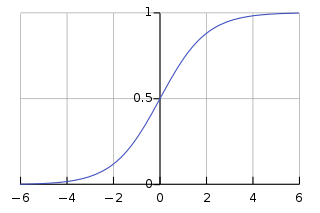
\includegraphics[width=.7\linewidth]{sigmoid}
	\caption{Hàm sigmoid}
\end{figure}

\noindent Hàm này có các tính chất sau:
\begin{itemize}
	\item Là hàm số liên tục nhận giá trị thực, bị chặn trong khoảng $(0, 1).$
	\item Hàm sigmoid có đạo hàm mọi nơi.
	\item Nếu coi điểm có tung độ là $0.5$ làm điểm phân chia thì các điểm càng xa điểm này về phía bên trái có giá trị càng gần 0. Ngược lại, các điểm càng xa điểm này về phía phải có giá trị càng gần 1.
\end{itemize}

\subsection{Xây dựng và tối ưu hàm mất mát}
\subsubsection{Xây dựng hàm mất mát}
Ta có thể giả sử rằng xác suất để một điểm dữ liệu $\textbf{x}_i$ rơi vào class 1 là $f(g(\theta, \textbf{x}_i))$ và rơi vào class 0 là $1-f(g(\theta, \textbf{x}_i))$. Để đơn giản, chọn hàm tuyến tính theo $\theta$ và $\textbf{x}_i$
$$g(\theta, \textbf{x}_i)=\theta_0+\theta_1x_{i1}+\theta_2x_{i2}+\cdots+\theta_nx_{in}=\theta^T\textbf{x}_i,$$ 
với $\theta=[\theta_0, \theta_1, \theta_2,\cdots,\theta_n]^T,\, \textbf{x}_i=[1, x_{i1}, x_{i2}, \cdots, x_{in}]^T\in \mathbb{R}^{(n+1)\times1}$. 
\\
Với mô hình được giả sử như vậy, với các điểm dữ liệu training, ta có thể viết như sau:
\begin{align}
	&P(y_i = 1 | \mathbf{x}_i; \theta) = f(\theta^T\mathbf{x}_i)=h_\theta(\textbf{x}_i) \label{1} \\
	&P(y_i = 0 | \mathbf{x}_i; \theta) = 1 - f(\theta^T\mathbf{x}_i)=1-h_\theta(\textbf{x}_i) \label{2}
\end{align}
trong đó $	P(y_i = 1 | \mathbf{x}_i; \theta)$ được hiểu là xác suất xảy ra sự kiện đầu ra $y_i=1$ khi biết tham số mô hình $\theta$ và dữ liệu đầu vào $\textbf{x}_i$.
\\ 
Mục đích của chúng ta là tìm các hệ số $\theta$ sao cho 
\begin{align*}
	&f(\theta^T\textbf{x}_i)\to 1 \text{ nếu } \textbf{x}_i\in \text{class 1}\\
	&f(\theta^T\textbf{x}_i)\to 0 \text{ nếu } \textbf{x}_i\in \text{class 0}
\end{align*}
%$f(\theta^T\textbf{x})$ càng gần với $1$ càng tốt với các điểm dữ liệu thuộc class 1 và càng gần với $0$ càng tốt với những điểm thuộc class 0.
Hai biểu thức \eqref{1} và \eqref{2} được viết gộp lại như sau:
$$P(y_i| \mathbf{x}_i; \theta) = h_\theta(\textbf{x}_i)^{y_i}(1 - h_\theta(\textbf{x}_i))^{1- y_i}.$$
Chúng ta muốn mô hình gần với dữ liệu training đã cho nhất, tức xác suất này đạt giá trị cao nhất.
\\
Xét toàn bộ dữ liệu training với $\mathbf{X} = [\mathbf{x}_1,\mathbf{x}_2, \dots, \mathbf{x}_n] \in \mathbb{R}^{d \times n}$ và $\mathbf{y} = [y_1, y_2, \dots, y_n]$, chúng ta cần tìm $\theta$ để biểu thức sau đây đạt giá trị lớn nhất:
$$\max_{\theta} P(\mathbf{y}|\mathbf{X}; \theta),$$
hay 
$$\theta = \arg\max_{\theta} P(\mathbf{y}|\mathbf{X}; \theta).$$
Bài toán tìm tham số để mô hình gần với dữ liệu nhất trên đây có tên gọi chung là bài toán maximum likelihood estimation với hàm số $P(\mathbf{y}|\mathbf{X}; \theta)$ được gọi là likelihood function. 
\\
Giả sử thêm rằng các điểm dữ liệu được sinh ra một cách ngẫu nhiên độc lập với nhau (independent), ta có thể viết:
\begin{align*}
	P(\mathbf{y}|\mathbf{X}; \theta) &= \prod_{i=1}^m P(y_i| \mathbf{x}_i; \theta) \\
	&= \prod_{i=1}^m h_\theta(\textbf{x}_i)^{y_i}(1 - h_\theta(\textbf{x}_i))^{1- y_i}.
\end{align*}
Nhận xét: Khi $m$ lớn, tích của $m$ số nhỏ hơn $1$ có thể dẫn tới sai số trong tính toán vì tích là một số quá nhỏ. Một phương pháp thường được sử dụng đó là lấy logarit tự nhiên (cơ số e) của likelihood function biến phép nhân thành phép cộng và để tránh việc số quá nhỏ. Sau đó lấy ngược dấu để được một hàm và coi nó là hàm mất mát. Lúc này bài toán tìm giá trị lớn nhất (maximum likelihood) trở thành bài toán tìm giá trị nhỏ nhất của hàm mất mát (hàm này còn được gọi là negative log likelihood):
\begin{align*}
	J(\theta) &= -\log P(\mathbf{y}|\mathbf{X};\theta) \\
	&= -\sum_{i=1}^m \left[y_i \log h_\theta(\textbf{x}_i) + (1-y_i) \log (1 - h_\theta(\textbf{x}_i))\right].
\end{align*}
Dựa vào \textbf{phần 1.4}, chúng ta sẽ tinh chỉnh hàm loss function ở trên và sẽ thu được:
\begin{align}\label{3}
	J_\lambda(\theta) = -\frac{1}{m}\sum_{i=1}^m \left[y_i \log h_\theta(\textbf{x}_i) + (1-y_i) \log (1 - h_\theta(\textbf{x}_i))\right]+\frac{\lambda}{2m}\sum_{j=1}^{n}\theta_j^2.
\end{align}
Lưu ý: Thành phần thứ 2 của \eqref{3} không có $\theta_0$.
\subsubsection{Tối ưu hàm mất mát}
Chúng ta sẽ sử dụng Gradient Descent với Momentum để giải bài toán tối ưu hàm mất mát \eqref{3}. Quy tắc cập nhật là:
$$\textbf{v} = \gamma\textbf{v} - \eta \nabla_{\theta} J(\theta),$$
$$\theta=\theta-\textbf{v}.$$
trong đó
\begin{align*}
	&\frac{\partial J_\lambda(\theta)}{\partial \theta_0}=\frac{1}{m}\sum_{i=1}^m\left(h_\theta(\textbf{x}_i)-y_i\right)x_{i0},\\
	&\frac{\partial J_\lambda(\theta)}{\partial \theta_j}=\frac{1}{m}\sum_{i=1}^m\left(h_\theta(\textbf{x}_i)-y_i\right)x_{ij}+\frac{\lambda}{m}\theta_j, \; j=1, 2, ..., n.
\end{align*}
\newpage
\section{Ví dụ minh họa}
\textit{\textbf{Mô tả dữ liệu}}:
\\
Dữ liệu là một bảng gồm $162,508$ hàng và $5$ cột, trong đó mỗi hàng tương ứng với 1 mẫu tàu. 
\\
Cột 1 chỉ có giá trị $0$ hoặc $1$, trong đó 0 = tàu cá và 1 = tàu khác (không phải tàu cá). Các cột 2, 3, 4, 5 là các số liệu tương ứng cho từng mẫu, tức là mỗi mẫu tàu (mỗi hàng) sẽ có 3 đại lượng đặc trưng là vận tốc (speed), công suất (power), range (cự ly) và số lượng điểm dấu (plotCount).
\\
Tập training sẽ gồm $130,006$ hàng đầu tiên và tập test là sẽ những hàng còn lại.
\begin{table}[h!]
	\centering
	\begin{tabular}{ |c|c|c| } 
		\hline
		\begin{tabular}{@{}c@{}}\quad$\lambda$ \\ $\eta$\quad\quad\end{tabular}& $0$ & $1000$ \\ 
		\hline
		$0.05$ & \begin{tabular}{@{}c@{}}accuracy: $0.9580$ \\ iteration: $11,800$ \end{tabular} & \begin{tabular}{@{}c@{}}accuracy: $0.9636$ \\ iteration: $1,100$ \end{tabular} \\
		\hline 
		$0.1$ & \begin{tabular}{@{}c@{}}accuracy: $0.9580$ \\ iteration: $6,400$ \end{tabular} & \begin{tabular}{@{}c@{}}accuracy: $0.9636$ \\ iteration: $600$ \end{tabular} \\ 
		\hline
	\end{tabular}
	\caption{Độ chính xác và số vòng lặp}
\end{table}


\end{document}
